\documentclass[10pt,hyperref={CJKbookmarks=true},xcolor=dvipsnames,aspectratio=169]{beamer}
\usetheme[navigation]{UMONS}
\usepackage[utf8]{inputenc}
\usepackage{verbatim}
\usepackage{ctex}

\title[国际经济学]{国际经济学}
\subtitle{贸易政策的国际协调:WTO与PTA}
\author{鲁晓东}
\institute[]{%
	岭南学院\hspace{2em}中山大学
	\\[4ex]
	
\includegraphics[height=8ex]{fig/lingnanlogo}\hspace{2em}%
	
\includegraphics[height=8.5ex]{fig/sysu}
}
%------------section前展示一页----------
\AtBeginSection[] {     
	\begin{frame}        
	\tableofcontents[currentsection,hideallsubsections]    
\end{frame} 
}

%-------------subsection也展示一下----------
\AtBeginSubsection[]{

\frame<beamer>{ 
	
	\frametitle{Outline}   
	
	\tableofcontents[currentsection,currentsubsection] 
	
}

}
%---------------------------

%-----------一段一闪现-------
%\beamerdefaultoverlayspecification{<+->}
%这个功能基本不用

\begin{document}
\maketitle


\begin{frame}
\frametitle{提纲}
\tableofcontents
\end{frame}				%生成提纲页

%-----------正文开始----------------------

%\beamerdefaultoverlayspecification{<+->}
\section{贸易谈判的经济学分析}
\frame{
	\frametitle{International Negotiations}
	\begin{itemize}
		\item A US-centric history of trade milestones:
		\begin{itemize}
			\item 1930: Smoot-Harley Act
			\item 1932: Bilateral negotiations
			\item 1947: Multilateral negotiations (GATT)
			\item 1995: WTO
			\item 2015: TPP(quit for now)
		\end{itemize}
		\item US Tariff rates over the years
	\end{itemize}
 \centering 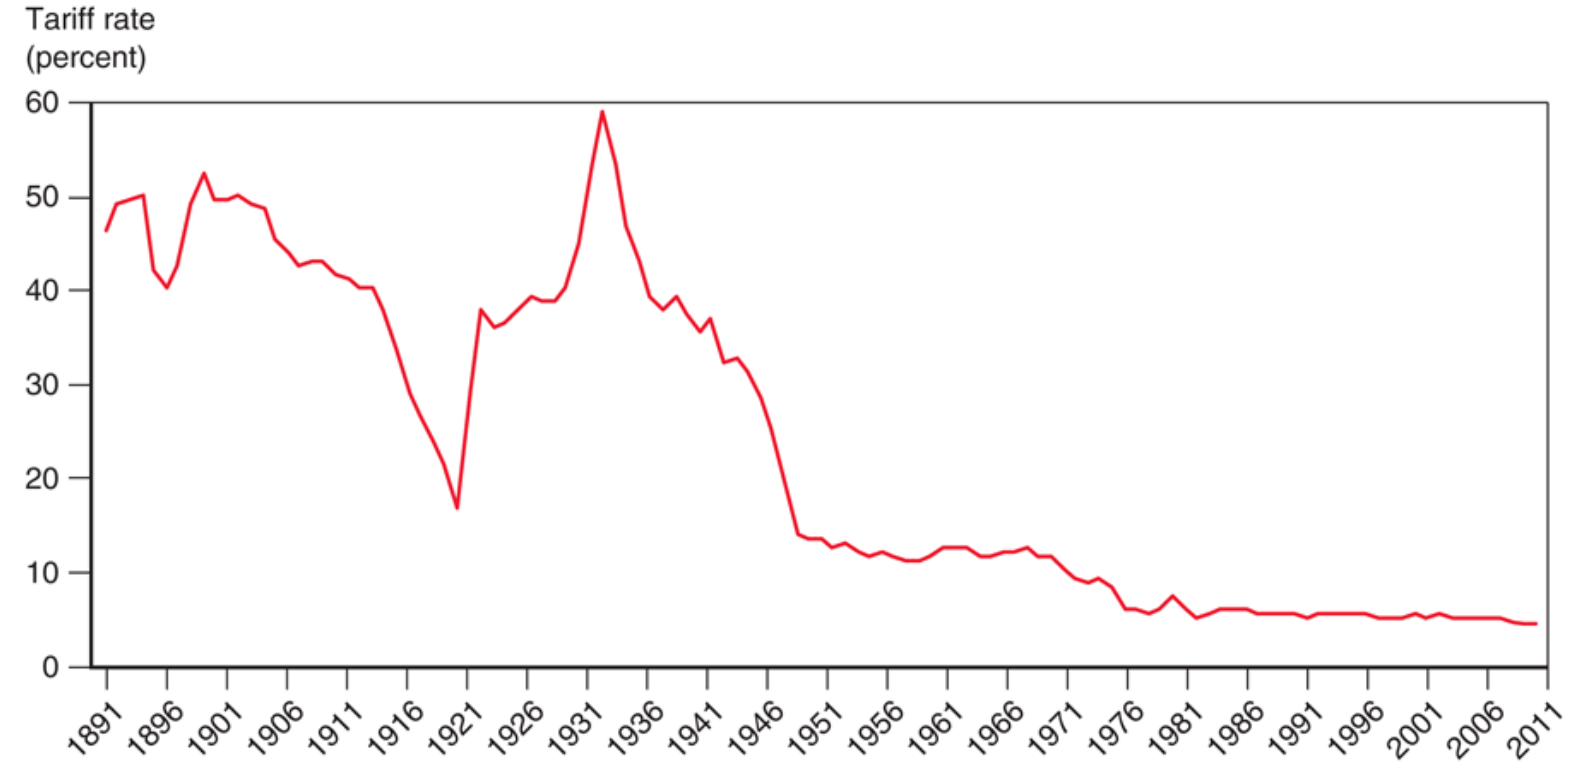
\includegraphics[scale=0.16]{fig/politic/tariff_rates_US.png}
}

\begin{frame}{Benefits of Trade Negotiations}
\begin{itemize}
	\item Other countries will demand less protection from Home
	\item Nice way to counter special interests at Home by getting exporter involved
	\item Can also help avoid a trade war
\end{itemize}
\end{frame}

\frame{
\frametitle{Trade War 的经济学分析 }
\begin{table}
	\begin{tabular}{c c||c c|c c||}
		& & \multicolumn{4}{c||}{\textcolor{blue}{\textbf{China}}}\\\hline\hline
		& &   \multicolumn{2}{c|}{Free Trade} & \multicolumn{2}{c||}{Protection}\\\hline
		\textcolor{red}{\textbf{US}}& Free trade &  &     &  &      \\\hline
		&  &       &  & &      \\\hline\hline
	\end{tabular}
\end{table}
}

\frame{
\frametitle{Trade War }
\begin{table}
	\begin{tabular}{c c||c c|c c||}
		& & \multicolumn{4}{c||}{\textcolor{blue}{\textbf{China}}}\\\hline\hline
		& &   \multicolumn{2}{c|}{Free Trade} & \multicolumn{2}{c||}{Protection}\\\hline
		\textcolor{red}{\textbf{US}}& Free trade &  & \textcolor{blue}{10B }     &  &   \textcolor{blue}{20B }   \\\hline
		&  &       &  & &       \\\hline\hline
	\end{tabular}

\end{table}
\begin{itemize}
	\item 在其他国家政策给定的情况下,任何一国政府都会选择保护政策
	
\end{itemize}
}

\frame{
\frametitle{Trade War }
\begin{table}
	\begin{tabular}{c c||c c|c c||}
		& & \multicolumn{4}{c||}{\textcolor{blue}{\textbf{China}}}\\\hline\hline
		& &   \multicolumn{2}{c|}{Free Trade} & \multicolumn{2}{c||}{Protection}\\\hline
		\textcolor{red}{\textbf{US}}& Free trade &  & \textcolor{blue}{10B }     &  &   \textcolor{blue}{$\underline{20B }$}   \\\hline
		&  &       &  & &        \\\hline\hline
	\end{tabular}
\end{table}
}

\frame{
\frametitle{Trade War }
\begin{table}
	\begin{tabular}{c c||c c|c c||}
		& & \multicolumn{4}{c||}{\textcolor{blue}{\textbf{China}}}\\\hline\hline
		& &   \multicolumn{2}{c|}{Free Trade} & \multicolumn{2}{c||}{Protection}\\\hline
		\textcolor{red}{\textbf{US}}& Free trade &  & \textcolor{blue}{10B }     &  &   \textcolor{blue}{$\underline{20B }$}   \\\hline
		\textcolor{red}{\textbf{US}}&Protection  &       & \textcolor{blue}{-10B } & &  \textcolor{blue}{-5B }      \\\hline\hline
	\end{tabular}
\end{table}
}

\frame{
\frametitle{Trade War }
\begin{table}
	\begin{tabular}{c c||c c|c c||}
		& & \multicolumn{4}{c||}{\textcolor{blue}{\textbf{China}}}\\\hline\hline
		& &   \multicolumn{2}{c|}{Free Trade} & \multicolumn{2}{c||}{Protection}\\\hline
		\textcolor{red}{\textbf{US}}& Free trade &  & \textcolor{blue}{10B }     &  &   \textcolor{blue}{$\underline{20B }$}   \\\hline
		\textcolor{red}{\textbf{US}}&Protection  &       & \textcolor{blue}{-10B } & &  \textcolor{blue}{$\underline{-5B }$}      \\\hline\hline
	\end{tabular}
\end{table}
\begin{itemize}
	\item 即使各国政府单独行动,采取保护政策也会使损失更小
	\item 博弈论中把这种策略称为什么?
	
\end{itemize}
}





\frame{
\frametitle{Trade War }
\begin{table}
	\begin{tabular}{c c||c c|c c||}
		& & \multicolumn{4}{c||}{\textcolor{blue}{\textbf{China}}}\\\hline\hline
		& &   \multicolumn{2}{c|}{Free Trade} & \multicolumn{2}{c||}{\textcolor{blue}{Protection}}\\\hline
		\textcolor{red}{\textbf{US}}& Free trade & \textcolor{red}{10B } & \textcolor{blue}{10B }     &  &   \textcolor{blue}{$\underline{20B }$}   \\\hline
		\textcolor{red}{\textbf{US}}&Protection  &  \textcolor{red}{20B }     & \textcolor{blue}{-10B } & &  \textcolor{blue}{$\underline{-5B }$}      \\\hline\hline
	\end{tabular}
\end{table}
}


\frame{
\frametitle{Trade War }
\begin{table}
	\begin{tabular}{c c||c c|c c||}
		& & \multicolumn{4}{c||}{\textcolor{blue}{\textbf{China}}}\\\hline\hline
		& &   \multicolumn{2}{c|}{Free Trade} & \multicolumn{2}{c||}{\textcolor{blue}{Protection}}\\\hline
		\textcolor{red}{\textbf{US}}& Free trade & \textcolor{red}{10B } & \textcolor{blue}{10B }     &  &   \textcolor{blue}{$\underline{20B }$}   \\\hline
		\textcolor{red}{\textbf{US}}&Protection  &  $\textcolor{red}{\underline{20B }}$     & \textcolor{blue}{-10B } & &  \textcolor{blue}{$\underline{-5B }$}      \\\hline\hline
	\end{tabular}
\end{table}
}


\frame{
\frametitle{Trade War }
\begin{table}
	\begin{tabular}{c c||c c|c c||}
		& & \multicolumn{4}{c||}{\textcolor{blue}{\textbf{China}}}\\\hline\hline
		& &   \multicolumn{2}{c|}{Free Trade} & \multicolumn{2}{c||}{\textcolor{blue}{Protection}}\\\hline
		\textcolor{red}{\textbf{US}}& Free trade & \textcolor{red}{10B } & \textcolor{blue}{10B }     &  \textcolor{red}{$\underline{-10B }$} &   \textcolor{blue}{$\underline{20B }$}   \\\hline
		\textcolor{red}{\textbf{US}}&Protection  &  $\textcolor{red}{\underline{20B }}$     & \textcolor{blue}{-10B } & \textcolor{red}{$\underline{-5B }$}&  \textcolor{blue}{$\underline{-5B }$}      \\\hline\hline
	\end{tabular}
\end{table}
}


\frame{
\frametitle{Trade War }
\begin{table}
	\begin{tabular}{c c||c c|c c||}
		& & \multicolumn{4}{c||}{\textcolor{blue}{\textbf{China}}}\\\hline\hline
		& &   \multicolumn{2}{c|}{Free Trade} & \multicolumn{2}{c||}{\textcolor{blue}{Protection}}\\\hline
		\textcolor{red}{\textbf{US}}& Free trade & \textcolor{red}{10B } & \textcolor{blue}{10B }     &  \textcolor{red}{$\underline{-10B }$} &   \textcolor{blue}{$\underline{20B }$}   \\\hline
		\textcolor{red}{\textbf{US}}& \textcolor{red}{Protection}  &  $\textcolor{red}{\underline{20B }}$     & \textcolor{blue}{-10B } & \textcolor{red}{$\underline{-5B }$}&  \textcolor{blue}{$\underline{-5B }$}      \\\hline\hline
	\end{tabular}
\end{table}

\begin{itemize}
	\item 博弈论中把这种情形称为什么?
	\item 如何避免出现这种情况,或者说避免出现这种情形的唯一出路是什么?
		
\end{itemize}
\begin{block}{任志强谈中美贸易战}
	世界上凡愿意打开大门的国家,都谈得成,不想打开大门的,都谈不成
\end{block}
}


\frame{
\frametitle{"Odysseus and the Sirens" (1)}
\textit{But if you wish to listen, let the men tie you in the lugger, hand
	and foot, back to the mast, lashed to the mast,
	so you may hear those harpies' thrilling voices...}[Homer, Odyssey]
\begin{figure}
	\centering
	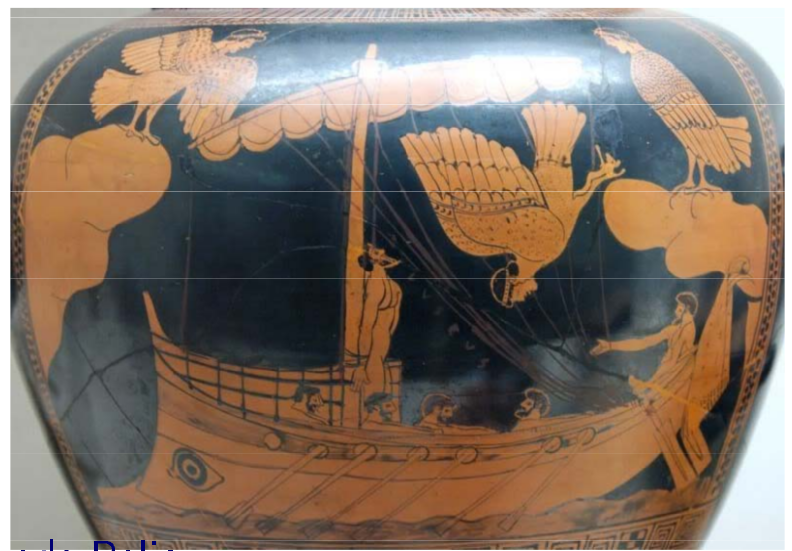
\includegraphics[width=0.5\textwidth]{fig/politic/ulysses.png}
\end{figure}
}

\frame{
\frametitle{"Odysseus and the Sirens" (2)}
If countries can establish a binding agreement to maintain free trade, both can avoid the temptation of protection and both can be made better off.
$\Rightarrow$ World Trade Organization (WTO)
\begin{enumerate}
	\item Reduction of tariff rates 
	\item Binding
	\item Prevention of non-tariff barriers
\end{enumerate}
}

\begin{frame}{Trade War}
\begin{itemize}
\item Side note: Prisoner's dilemma not as bad if repeated
\item How would does WTO affect the one-shot prisoner's dilemma?
\end{itemize}
\end{frame}

\frame{
\frametitle{Trade War }
\begin{table}
\begin{tabular}{c c||c c|c c||}
	& & \multicolumn{4}{c||}{\textcolor{blue}{\textbf{China}}}\\\hline\hline
	& &   \multicolumn{2}{c|}{Free Trade} & \multicolumn{2}{c||}{\textcolor{blue}{Protection}}\\\hline
	\textcolor{red}{\textbf{US}}& Free trade & \textcolor{red}{10B } & \textcolor{blue}{10B }     &  \textcolor{red}{$\underline{-10B }$} &   \textcolor{blue}{$\underline{5B }$}   \\\hline
	\textcolor{red}{\textbf{US}}& \textcolor{red}{Protection}  &  $\textcolor{red}{\underline{5B }}$     & \textcolor{blue}{-10B } & \textcolor{red}{$\underline{-5B }$}&  \textcolor{blue}{$\underline{-5B }$}      \\\hline\hline
\end{tabular}
\end{table}
}
\section{国际贸易协定的历史与现状}

\begin{frame}{History of Trade Agreements}
\begin{itemize}
	\item For most of history trade impediments had existed
	even within countries
	\item A famous early trade agreement was the Zollverein德意志关税同盟,
	a customs union between German states signed in
	1834
	\item Other agreements between countries/empires
	were signed in the 19th century, the most
	famous of which being the Cobden–Chevalier
	Treaty of 1860(1860年英法签订《柯布登条约》)
	\item 该条约中最为精巧的设计来自“最惠国待遇”
\end{itemize}

\end{frame}

\begin{frame}{Backlash in the Interwar Period}
\begin{columns}
	\begin{column}{0.6\textwidth}
		\begin{itemize}
			\item Tensions among countries rose after WWI and with
			the advent of the great depression many countries
			turned to protectionism
			\item In 1930, the U.S. passed a very stringent tariff law,
			the \structure{Smoot-Hawley Act} (tariffs rose and US trade
			fell)
			\begin{itemize}
				\item Very soon, the government decided this
				tariff was a bad idea
				\item However, special interests protected by the
				tariff made it very difficult to repeal
			\end{itemize}
		\end{itemize}
	\end{column}
	\begin{column}{0.4\textwidth}
		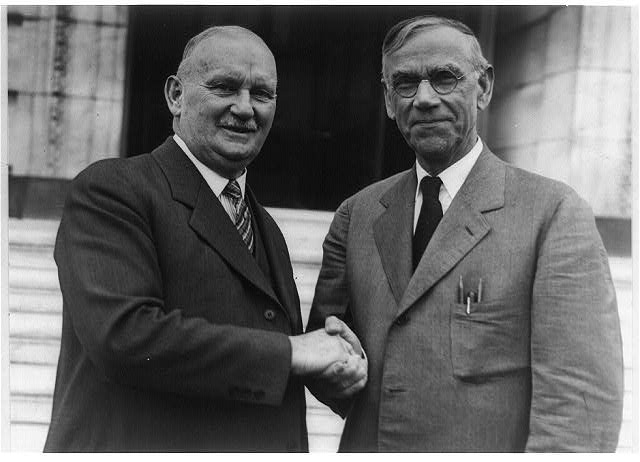
\includegraphics[scale=0.28]{fig/politic/smoot}
	\end{column}
\end{columns}
	
\end{frame}

\begin{frame}{History of Trade Agreements(cted.)}
	\begin{itemize}
		\item 	The initial solution to this problem was bilateral
		negotiations, where concessions to US exporters
		were traded for reductions in US tariffs
		\item This was feasible, as it balanced the interests of
		exporters against those of importers
		\item The average duty on US imports fell from 59\% in
		1932 to 25\% in 1945
		\item Multilateral negotiations began after WWII ended
		\begin{itemize}
			\item A body called the International Trade Organization was			proposed 
		\end{itemize}
		
	\end{itemize}
\end{frame}

\begin{frame}{History of Trade Agreements (cted.)}
	\begin{itemize}
		\item The ITO ran into strong political opposition, especially
		in the U.S., and in fact was never established
		\item Instead, 23 countries began trade negotiations under
		some provisional rules known as the General
		Agreement on Tariffs and Trade (GATT)
		\item Eight rounds of trade negotiations were carried out
		under these rules until the final (Uruguay) round
		established the WTO in 1995
		\item Over this 50-year period, restrictions on trade fell and
		the volume of trade rose considerably
	\end{itemize}
\end{frame}

\begin{frame}
\centering 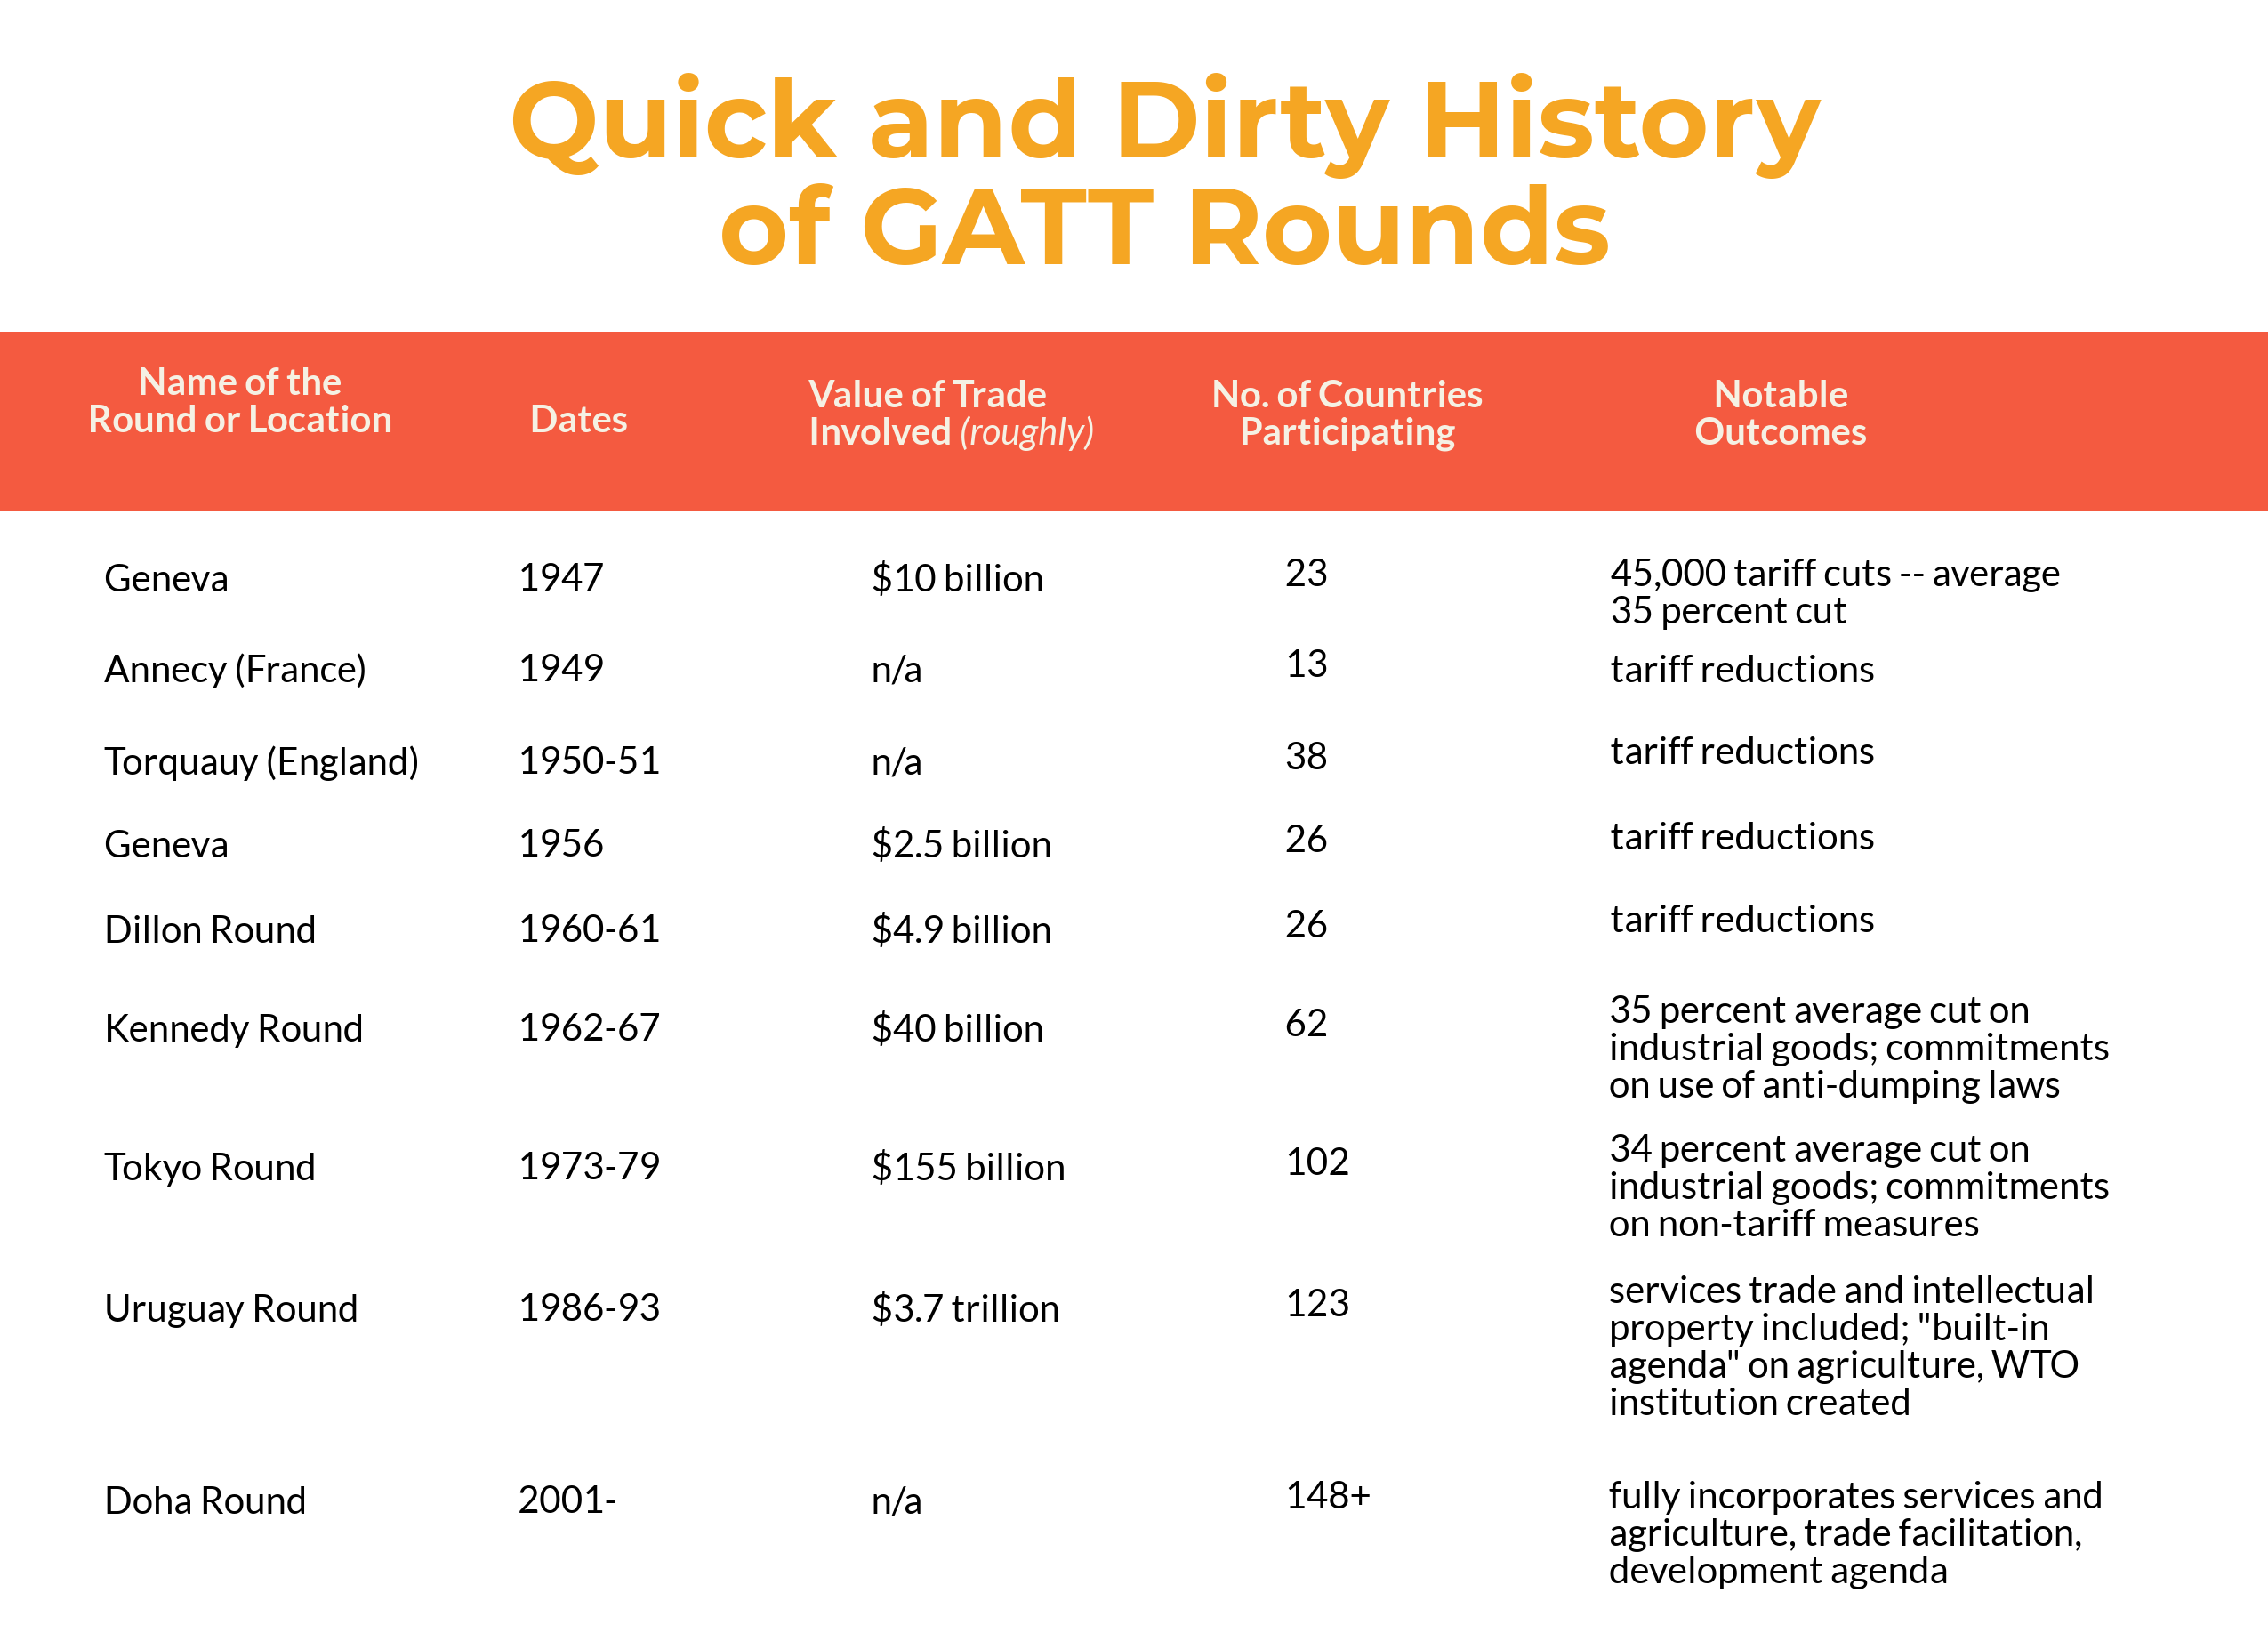
\includegraphics[scale=0.12]{fig/politic/gatt}
\end{frame}


\begin{frame}{The GATT and the WTO}
WTO negotiations address trade restrictions in at least 3 ways:	\begin{enumerate}
		\item \structure{Reducing tariff rates} through multilateral negotiations杠杆
		\item \structure{Binding tariff rates}: a tariff is “bound” by having the
		imposing country agree not to raise it in the future棘轮
		\item \structure{Eliminating nontariff barriers}: quotas and export subsidies		are changed to tariffs because the costs of tariff protection are		more apparent and easier to negotiate
		\begin{itemize}
			\item Subsidies for agricultural exports are an exception
			\item Exceptions are also allowed for “market disruptions” caused
			by a surge in imports
		\end{itemize}
		
	\end{enumerate}
\end{frame}

\begin{frame}{The WTO}
The WTO differs from GATT in several ways
	\begin{enumerate}
		\item 缔约国-成员
		\item It applies not just to trade in goods but also to trade in
		services (though this has not yet had much impact)
		\item It has taken up the issue of intellectual property rights
		through an agreement on the Trade-Related Aspects
		of Intellectual Property (TRIPS)
		\item It has a formal \textbf{\textcolor{red}{dispute settlement procedure}}
	\end{enumerate}

\end{frame}

\begin{frame}{The Dispute Settlement Procedure}
	\begin{itemize}
		\item Under GATT, even if rulings were made against
		some countries for particular actions, there was no
		enforcement mechanism
		\item The WTO organizes panels of experts to hear cases,
		and who make rulings relatively quickly
		\item The injured parties are then allowed to impose
		restrictions on the country in violation (e.g., U.S.
		steel)
	\end{itemize}
\end{frame}

\begin{frame}{The Administrative Structure of WTO}
\centering 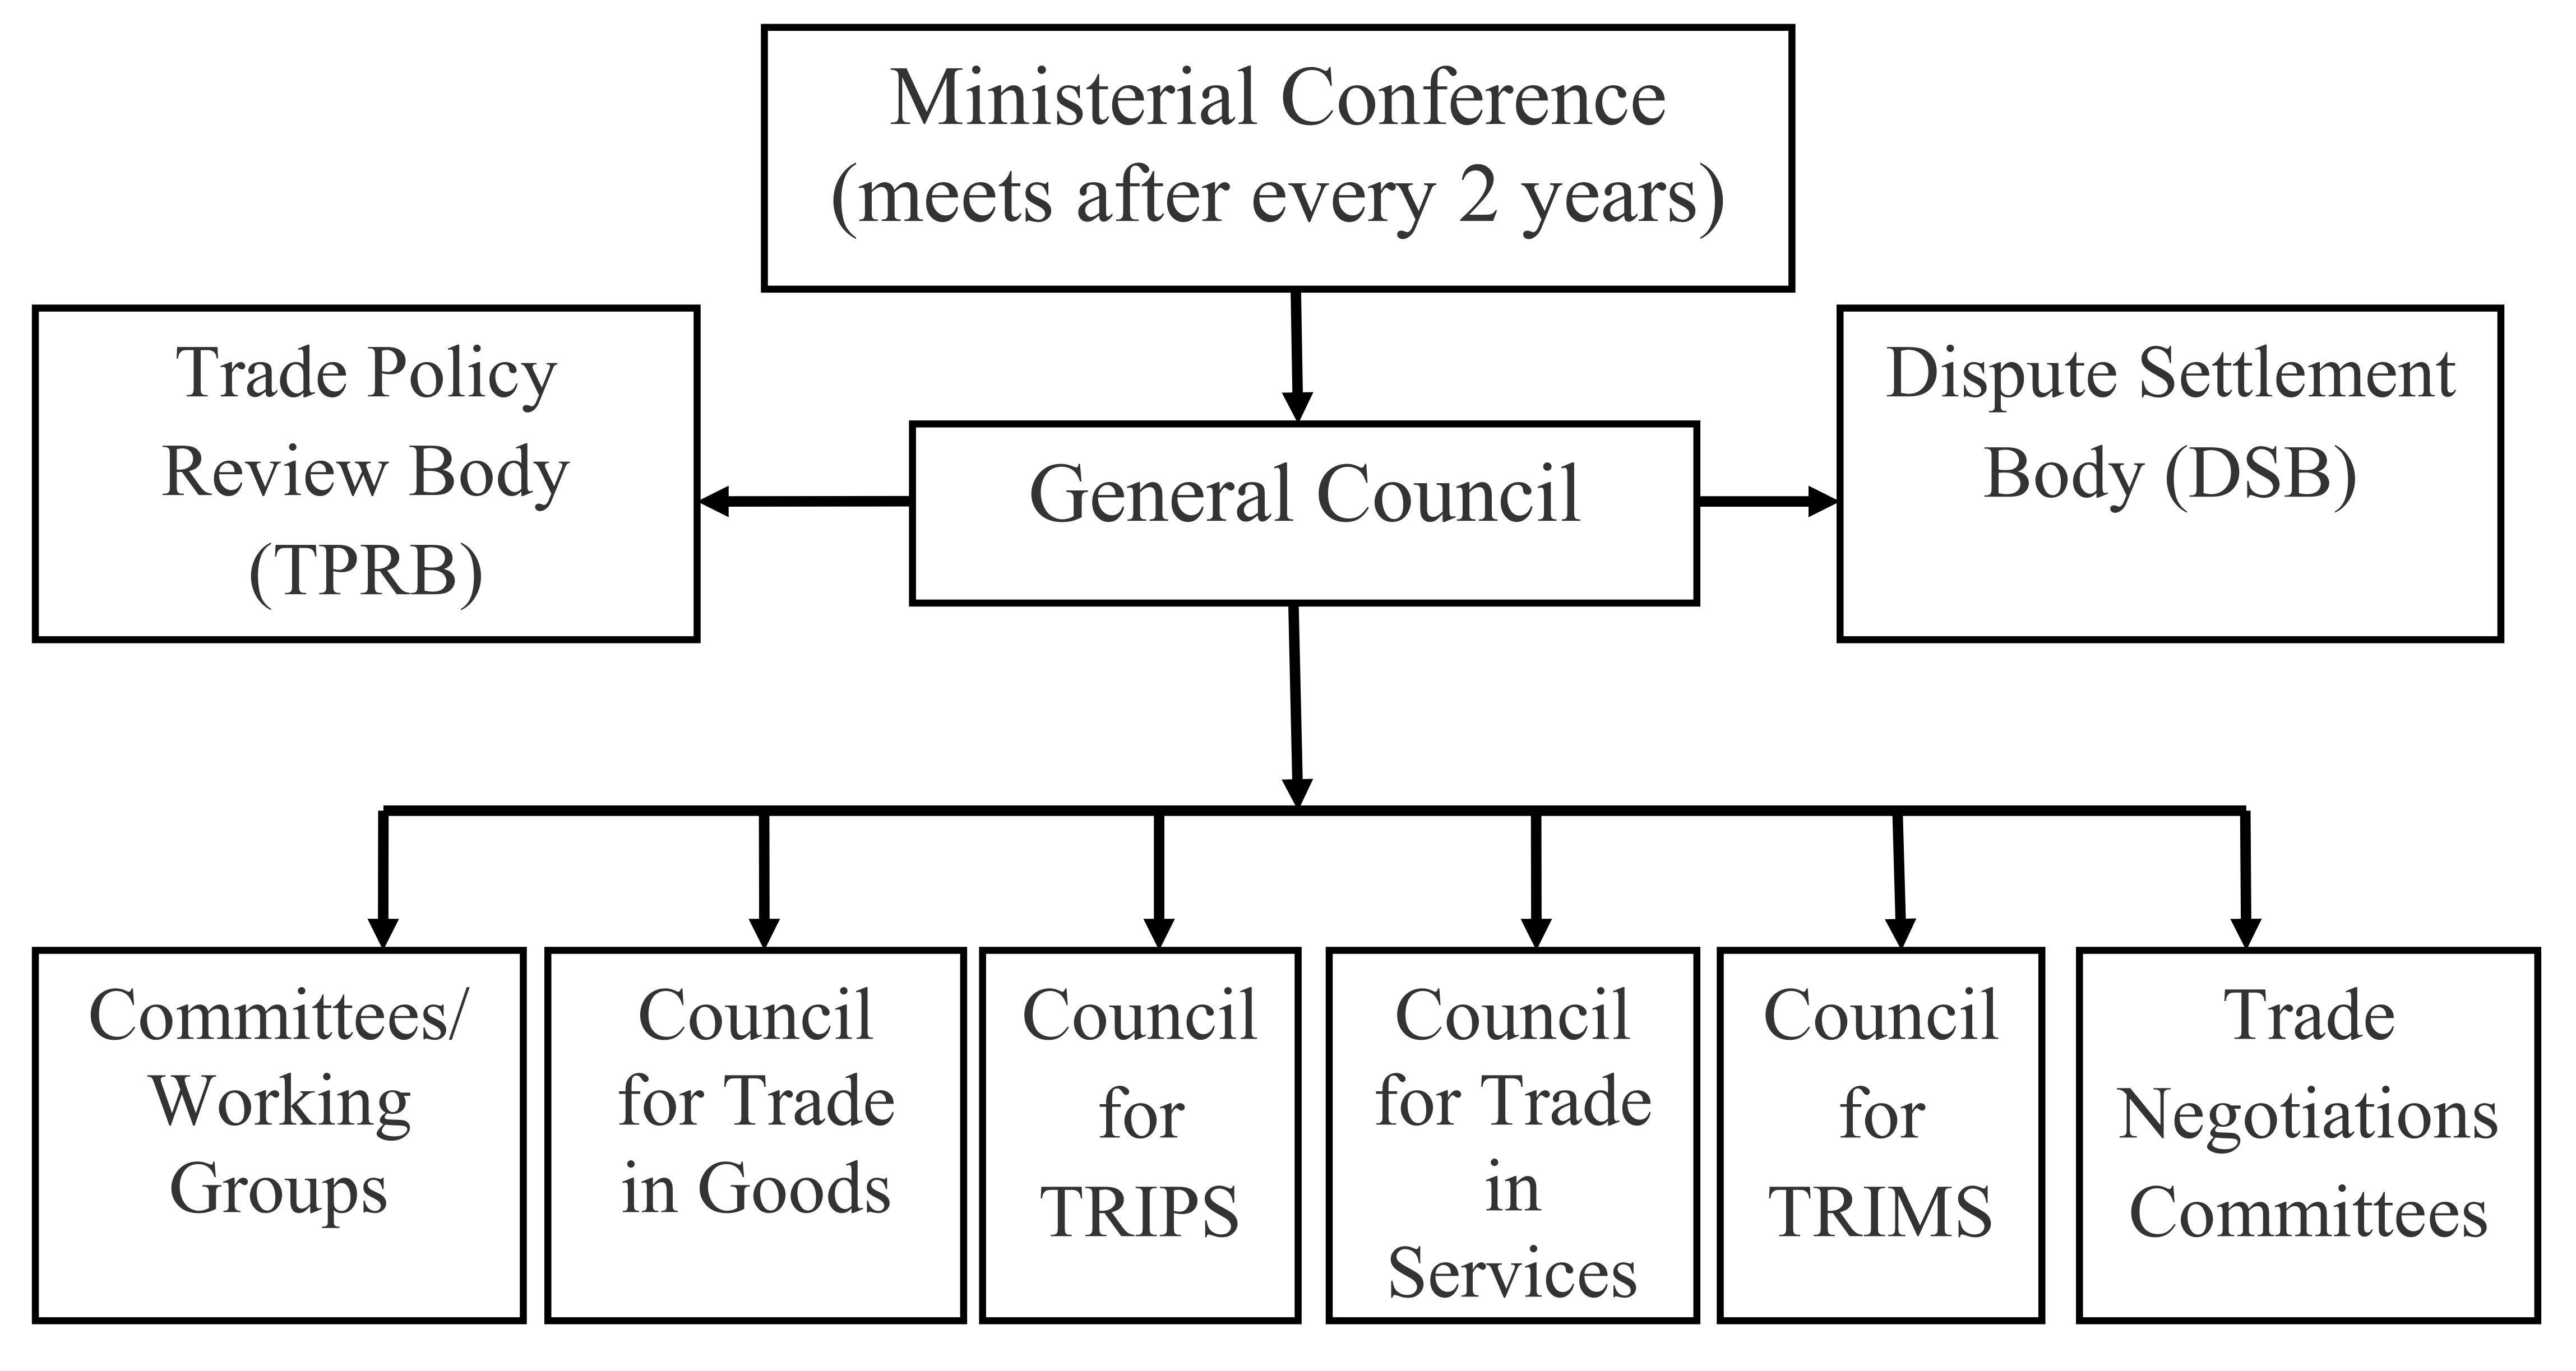
\includegraphics[scale=0.08]{fig/politic/wto2}
\end{frame}

\begin{frame}{The Doha Round}
	\begin{itemize}
		\item 	In 2001, a new round of negotiations was started in
		Doha, Qatar, but these negotiations have not yet
		produced an agreement
		\item Part of the reason for this is that the potential gains
		from further liberalization are modest
		\item  The sectors that are left to liberalize (agriculture,
		textiles, clothing) are particularly politically sensitive
		\item It was harder to generate Pareto improvements for all
		countries involved (Brazil and India complained)
	\end{itemize}
\end{frame}

\begin{frame}{The Doha Round}
\centering 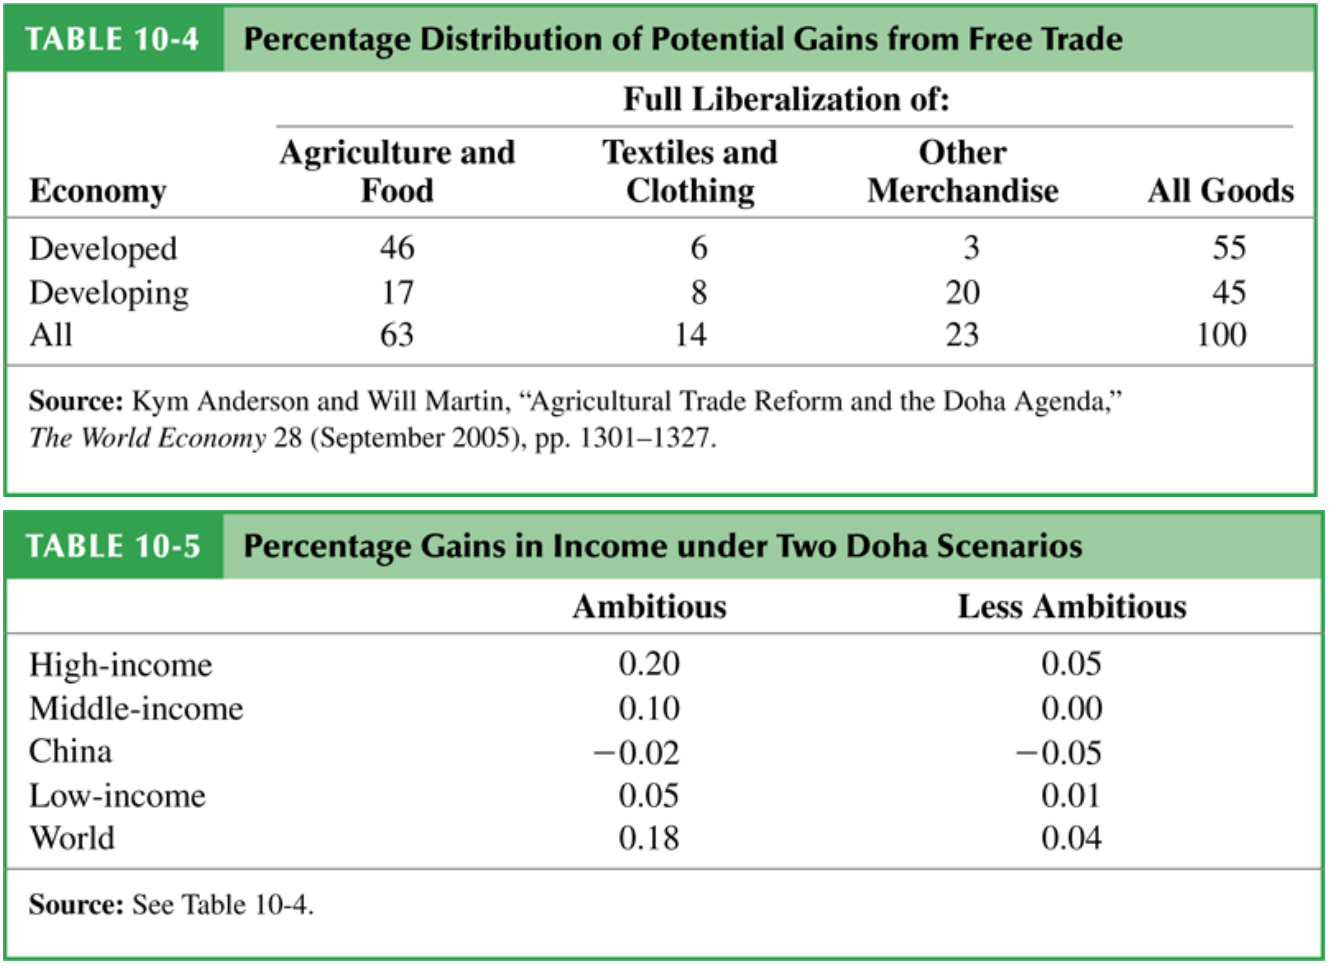
\includegraphics[scale=0.3]{fig/politic/doha1}
\end{frame}

\begin{frame}{Agricultural Subsidies and LDCs}
\begin{itemize}
	\item 	Rich countries protect textiles and agriculture, where LDCs
	might have comparative advantage
	\item This lowers world prices and can be quite harmful for LDCs
	that are large exporters of these goods
	\item For example, the US and EU heavily subsidize domestic
	cotton growers
	\begin{itemize}
		\item In 2001-2 US government subsidies to America’s 25,000 cotton
		farmers amounted to \$160,000 per farmer (\$4 billion total)
		\item Since the mid-1990s cotton prices have fallen by half
		\item This has had a big impact on some of the world’s other cotton
		producers
		\item US subsidies cost some countries more than 1\% of their GDP per year
		\item But other countries benefit (cotton-importing countries)
	\end{itemize}
	
\end{itemize}
\end{frame}


\begin{frame}{The Doha Round}
\centering 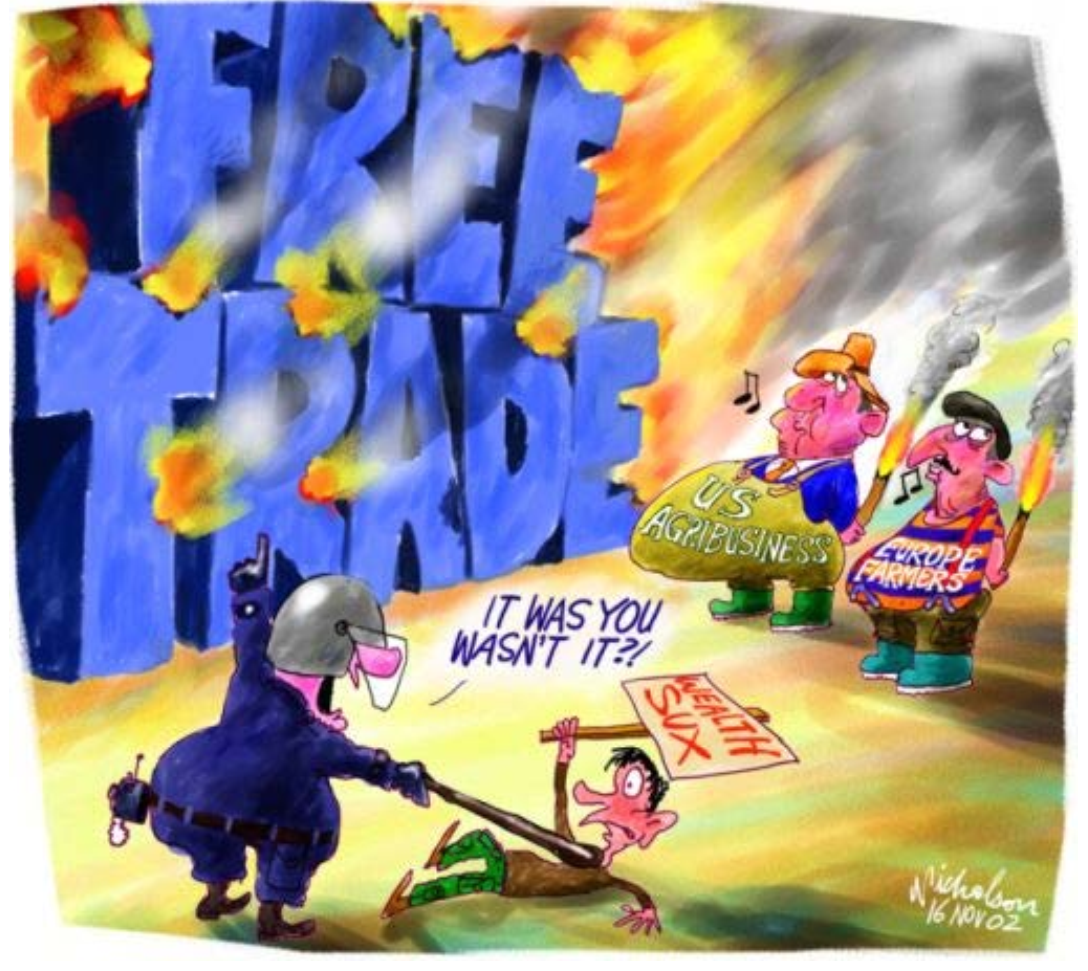
\includegraphics[scale=0.35]{fig/politic/doha2}
\end{frame}



\section{Preferential Trade Agreements特惠贸易协定}

\frame{
\frametitle{Preferential Trade Agreement}
\begin{itemize}
\item Under the GATT and WTO, reductions in tariff rates
are nondiscriminatory (they must apply to all members)
\item “Most Favored Nation” status implies that a country
receives the minimum tariff applied to all potential
importers
\item Only allowed under WTO if totally eliminate tariffs between partners
\end{itemize}
\begin{enumerate}
\item \textbf{free trade area:} an agreement that allows free trade among members, but each member can have its own trade policy towards non-member countries (e.g., NAFTA)
\item \textbf{custom unions:} an agreement that allows free trade among members and requires a common external trade policy towards non-member countries. (e.g., European Union)
\end{enumerate}
\begin{itemize}
\item Surprisingly, entering a free trade area can make a country worse off!
\item Some estimate that Mexico actually was made worse off by NAFTA
\end{itemize}
}

\begin{frame}
\centering 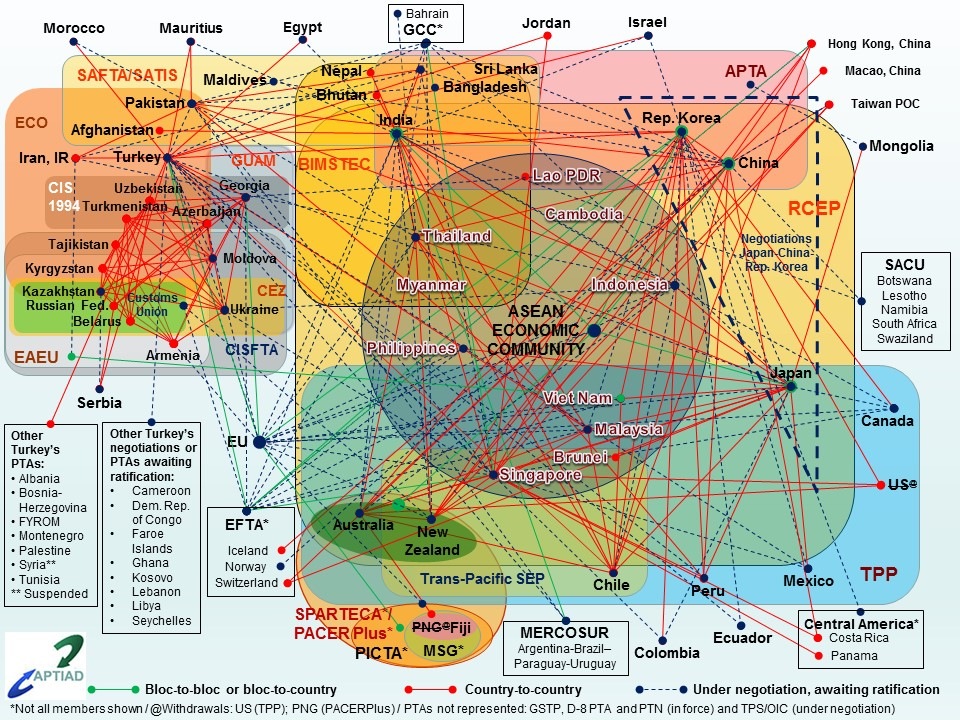
\includegraphics[scale=0.45]{fig/politic/noodlebowl}
\end{frame}

\frame{
\frametitle{Trade Creation vs. Trade Diversion}
	\begin{itemize}
		\item Are preferential trading agreements necessarily good
		for national welfare?
		\item No, it is possible that national welfare decreases
		under a preferential trading agreement
		\item How? Rather than gaining tariff revenue from
		inexpensive imports from world markets, a country
		may import expensive products from member
		countries but not gain any tariff revenue
			\begin{itemize}
				\item Trade Diversion may dominate Trade Creation 
				\item World Bank Report claimed that, for Mercosur, TD > TC
			\end{itemize}
	\end{itemize}
}

\frame{
\frametitle{Preferential Trade Agreement}
\begin{table}
\begin{tabular}{||l|c|c|c|c||}\hline \hline
& \textbf{UK} & \textbf{F} & \textbf{US} & \textbf{UK import from}\\ \hline
$p$ & 8 & 6 & 4 & US \\ \hline
\multicolumn{5}{||c||}{$1^{st}$ case}\\ \hline
$p+t$ & 8 & 11 & 9 & -\\
CU with F & 8 & 6 & 9 & F (trade creation)\\ \hline
\multicolumn{5}{||c||}{$2^{nd}$ case}\\ \hline
$p+t^{2}$ & 8 & 9 & 7 & US\\
CU with F & 8 & 6 & 7 & F (trade diversion)\\ \hline
\end{tabular}
\end{table}
}

\begin{frame}{The End of International Trade}
\begin{itemize}
	\item Today was a catch-all for trade policy issues
	\item The remainning issue is \structure{Trade and Development}. Absolutley it means a lot to every country. But I decided to skip it for its straightforward meaning. You can easily get the idea by reading the textbook yourselves.
	\item We Next time start International Finance section!
\end{itemize}
\end{frame}



\end{document}